%\immediate\write18{makeindex \jobname.nlo -s nomencl.ist -o \jobname.nls}
\documentclass[11pt]{article}
\usepackage[margin=0.5in]{geometry}
\usepackage[utf8]{inputenc}
\usepackage{subfig}
\usepackage{graphicx}
\usepackage{wrapfig}
\usepackage{amsmath}
\usepackage[version=4]{mhchem}
\usepackage{siunitx}
\usepackage{float}
\usepackage{algorithm}
\usepackage{algpseudocode}
\usepackage{placeins}
\usepackage{setspace}
\usepackage{longtable,tabularx}
\usepackage[colorlinks]{hyperref}% hyperlinks [must be loaded after dropping]
\usepackage{indentfirst}
\hypersetup{colorlinks,breaklinks,
citecolor = blue,
urlcolor=blue,
linkcolor=blue}
\usepackage[capitalise]{cleveref}

\RequirePackage[blocks]{authblk}
\renewcommand{\Authfont}{\normalsize\upshape}
\renewcommand{\Affilfont}{\normalsize\itshape}
\setlength{\affilsep}{0pt}

\bibliographystyle{aiaa}
\bibliographystyle{new-aiaa}
%\renewcommand{\bibfont}{\small}

%\usepackage{nomencl}% nomenclature generation via makeindex
\setlength\LTleft{0pt}

%\makenomenclature

\title{Offshore Wind Energy Simulator (OWENS) Code Basic Theory, Frames of Reference, and Inter-Module Coupling Methods}

\author{Brandon Ennis\footnote{Wind Pirate, Wind Energy Technologies, PO Box 5800, MS 1124.} , Brian Owens\footnote{Retired Wind Pirate, Retired Pirate People Area, PO Box 5800, MS 1124.} , Kevin R. Moore\footnote{R\&D, S\&E Mechanical Engineering, Wind Energy Technologies, PO Box 5800, MS 1124.} }

\affil{Sandia National Laboratories\footnote{Sandia National Laboratories is a multimission laboratory managed and operated by National Technology and Engineering
 Solutions of Sandia, LLC., a wholly owned subsidiary of Honeywell International, Inc., for the U.S. Department of Energy’s National Nuclear Security Administration under contract DE-NA-0003525}, Albuquerque, NM 87185}

\begin{document}

\maketitle

%\begin{abstract}
%
%\end{abstract}

%\printnomenclature


\section{Introduction}

The Offshore Wind Energy Simulator (OWENS) Code is a floating turbine-platform code capable of steady, unsteady, and modal analysis.  It is comprised of or coupled to many modules for aerodynamics, hydrodynamics, mooring dynamics, and at the core a finite element formulation for a gyric beams in a floating frame with an energy-conserving time-integration method for gyric systems and analytical flutter.

\textit{How} many of these items are used is not straightforward or a priori and can easily lead to confusion or mistake (like how the aerodynamics uses inflow data; is it just simple based on the mean hub velocity, or in the rotating blade frame of reference?  If the latter, what is that frame of reference so that we make sure we don't incorrectly map the vectors?) This document is intended as a developers guide for the intent of clearing up the relative ambiguity between the many moving and modular pieces.  It is not a full theory document or users guide.  (For full theory, please see Brian Owen's Dissertation~\cite{owens2013theoretical}.  For a users guide, please see the OWENS Users Guide, which will need to be included/released with the repository after it is cleaned up???)  Within this document, we give enough detail about the operations of the code, the frames of reference, and coupling methods to aid further development.  The following is a summary of the modules and what is included:

\begin{table}[htbp!]
\begin{center}
\caption{Module Level of Detail in This Document}
\begin{tabular}{|c| c c c|}
\hline
Module (With Source Link) & Code Theory & Frame of Reference & Coupling Method and I/O \\
\hline
\href{https://github.com/old-NWTC/InflowWind}{Turbulent Inflow} & N & Y & Y  \\
\href{https://gitlab.sandia.gov/8821-vawt-tools/VAWTAero.jl}{Aerodynamics} & N & Y & Y \\
\href{https://gitlab.sandia.gov/8821-vawt-tools/OWENS.jl}{Turbine Structures} & Y & Y & Y \\
Platform Structures & N & Y & Y \\
\href{https://gitlab.sandia.gov/8821-vawt-tools/PreComp.jl}{Sectional Properties}& N & Y & Y \\
\href{https://github.com/byuflowlab/Composites.jl}{Composites} & N & Y & Y \\
Hydrodynamics & N & Y & Y \\
Mooring & N & Y & Y \\
\hline

\end{tabular}
\end{center}
\end{table}

Code theory for the non-covered modules used can be found in the following locations: aerodynamics is actuator cylinder~\cite{ac} and/or double multiple streamtube~\cite{DMS}, with the possibility for CACTUS~\cite{cactus}.  Turbine structures is covered in the document as well as~\cite{owens2013theoretical}. Inflow, platform structures, hydrodynamics, and mooring are the respective openFAST modules~\cite{openFAST}.  Composite properties is PreComp~\cite{precomp}.  (Also include links to where the code and code theory can be found.)

%\begin{equation}
%\label{e:tau_1}
%    \tau_1 = \frac{\tau_{\text{near}} R_{\text{ref}}}{V_{\text{wakeOld}}}
%\end{equation}
%
%\begin{equation}
%\label{e:tau_2}
%    \tau_2 = \frac{\tau_{\text{far}}R_{\text{ref}}} {V_{\text{wakeOld}}}
%\end{equation}

\vspace{12pt}



\section{Basic Theory}

Due to the nonlinearity and non-closed-form nature of the floating turbine problem in both the design and temporal space, OWENS uses many types of iterative solution methods, specific to the physics involved.  These include Newton-Rapson or Direct Iteration for the beam elements, Loose or Gauss-Seidel iteration for the coupling between the modules, and p-k iteration for the modal flutter analysis.  \Cref{alg:Transient} gives an overview of the general code structure for transient analysis, with the main equations being solved and the relative location of the iteration loops.

%\vspace{12pt}
\begin{algorithm}
\caption{OWENS Transient Analysis General Algorithm}
\begin{spacing}{1.18}
\begin{algorithmic}[1]
\State Initialize simulation (all module parameters, meshing, composite properties, etc)
\State Initialize displacements and forces as 0
\For {$t \leftarrow 0:dt:t_{\text{max}} $}

	\While {norm(displacements$_{\text{guess}}$ - displacements) $>$ Tol}

		\State Get platform and mooring displacements from force
		\State Get driveshaft displacement from generator torque
		\State Get rotor speed, rotational displacement from generator torque, aero torque, and turbine inertia
		\State Get aero forces from rotor speed, position
		\State Get structural displacements and reaction forces from aero forces
		\While {residual $>$ Tol}
			\State Calculate effective force and stiffness from dynamic displacements
			\State Calculate displacements from effective force and stiffness
			\State Predict next iteration displacements from Newton-Rapson step
			\State residual = norm(new displacements - old displacements) / (new displacements)
		\EndWhile
		\State Update displacements$_\text{guess}$ with the calculated displacements
	\EndWhile
\EndFor

\end{algorithmic}
\end{spacing}
\label{alg:Transient}
\end{algorithm}
%\vspace{12pt}


%\vspace{12pt}
\begin{algorithm}
\caption{OWENS Steady/Static Analysis General Algorithm}
\begin{spacing}{1.18}
\begin{algorithmic}[1]

\State Initialize simulation (all module parameters, meshing, composite properties, etc)
\State Precompute (warm start) the Timoshenko beam elements
\State If static set rotation to zero, if steady set to steady value
\While {residual $>$ Tol}
	\State Get External Forces
	\State Calculate effective force and stiffness from dynamic displacements
	\State Calculate displacements from effective force and stiffness
	\State Predict next iteration displacements from Newton-Rapson step
	\State residual = norm(new displacements - old displacements) / (new displacements)
\EndWhile
\end{algorithmic}
\end{spacing}
\label{alg:Steady}
\end{algorithm}
%\vspace{12pt}


%\vspace{12pt}
\begin{algorithm}
\caption{OWENS Modal Analysis General Algorithm}
\begin{spacing}{1.18}
\begin{algorithmic}[1]

\State Initialize simulation (all module parameters, meshing, composite properties, etc)
\State Run Steady Analysis
\State Calculate Effective Mass, Stiffness, and Damping
\State Run Eigensolve

\end{algorithmic}
\end{spacing}
\label{alg:Modal}
\end{algorithm}
%\vspace{12pt}

%\vspace{12pt}
\begin{algorithm}
\caption{OWENS Flutter Analysis General Algorithm}
\begin{spacing}{1.18}
\begin{algorithmic}[1]
\State Initialize simulation (all module parameters, meshing, composite properties, etc)
\State Initialize displacements and forces as 0
\For each rotational speed
	\State Run Static Analysis
	\State Run Modal Analysis
	\For each mode
		\While {residual $>$ Tol}
			\State Get External Forces
			\State Calculate effective force and stiffness from dynamic displacements
			\State Calculate displacements from effective force and stiffness
			\State Predict next iteration displacements from Newton-Rapson step
			\State residual = abs(frequency$_\text{mode}$ - guess frequency)
		\EndWhile
	\EndFor
\EndFor

\end{algorithmic}
\end{spacing}
\label{alg:Flutter}
\end{algorithm}
%\vspace{12pt}


 The algorithm variables not previously defined are as follows: residual solution tolerance Tol, number of circumferential discretizations $N_{\theta}$,

\section{Global Frame of Reference}

\begin{figure}[H]
\centering
\vspace{-12pt}
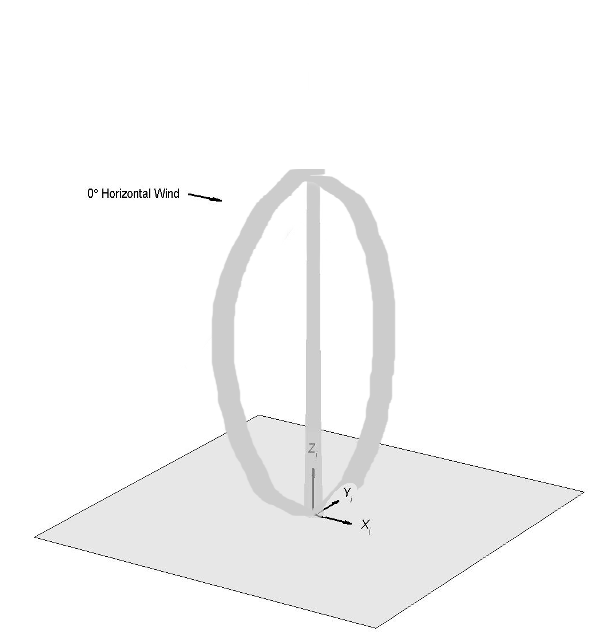
\includegraphics[trim={0 0 0 0},clip,width=0.5\textwidth]{./figs/global_FOR.png}
\vspace{-12pt}
\caption{Draft Global Frame of Reference, should be prettified.  Wind comes in from the left in the direction of the positive X-axis, the positive Y-axis is 90 degrees counter-clockwise to the X-axis.  Z-axis is vertical.  Positive rotations follow right hand rule.}
\label{fig:ac_velocities}
\end{figure}

\section{Inflow}

\begin{figure}[H]
\centering
\vspace{-12pt}
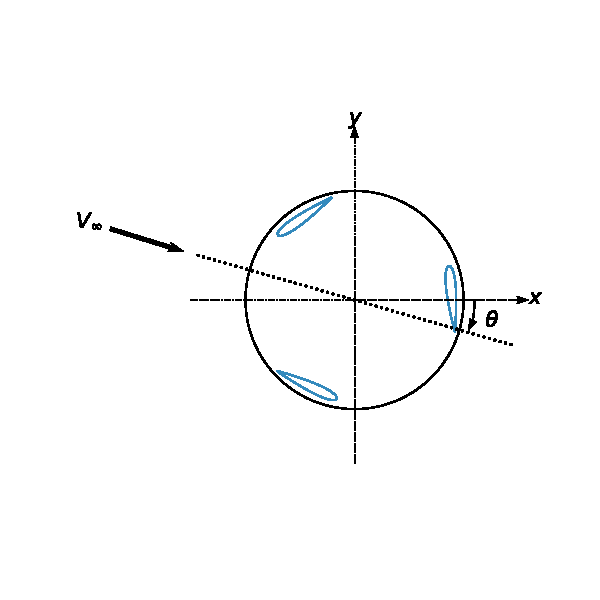
\includegraphics[trim={1.3cm 2.4cm .5cm 1.5cm},clip,width=0.5\textwidth]{./figs/inflow_wind}
\vspace{-12pt}
\caption{Wind frame of reference is the same as global.  Wind propagation angle is zero when aligned with the positive X-axis and clockwise positive, in the direction of the negative negative Y-axis.}
\label{fig:ac_velocities}
\end{figure}

\section{Aerodynamics}

\begin{figure}[H]
\centering
\vspace{-12pt}
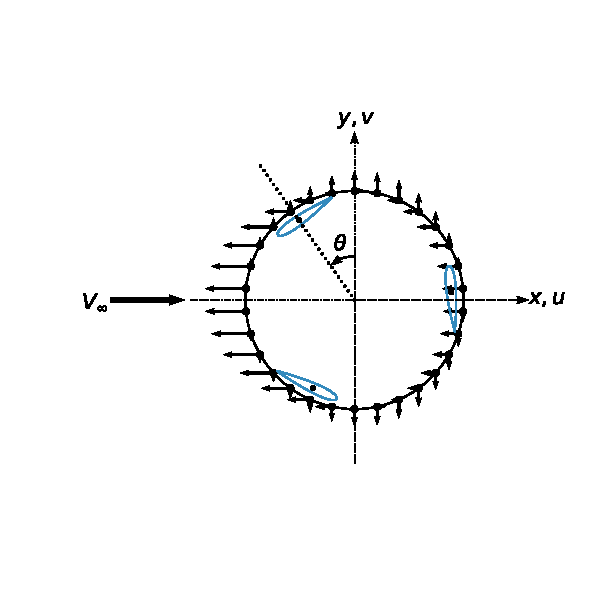
\includegraphics[trim={1.3cm 2.4cm .5cm 1.5cm},clip,width=0.5\textwidth]{./figs/vawt_slice}
\vspace{-12pt}
\caption{VAWT 2D section looking downwards with induced velocity \(w\) vector broken into \(u\) and \(v\) components depicted by arrows. Airfoils show example blade locations with dots aligning to the circumferential discretization.  Aero frame of reference is the same as global, however a blade is at 0 degrees azimuth when it is aligned with the Y-axis.  If an aero module is 2D, it is made quasi-3D by stacking slices from lower to higher in the Z-axis.}
\label{fig:ac_velocities}
\end{figure}

Note: CACTUS, does not fully follow this scheme and differs from the global frame of reference by switching the Y and Z axes for a VAWT.  Be careful with the geometry inputs; if the blade 1 starts out at the "south" position, as opposed to the north, then it will behave as though it were a north starting blade rotating clockwise, and the gust velocity will match (if the simple iec uniform gust is used).  All else follows the description above.

\subsection{Turbine Structures}

Rotating Frame of Reference, 6 DOF where 1 = turbine vertical force, 2 = turbine 2D slice tangential force, 3 = turbine 2D slice normal force, 4 = blade M25 twisting moment, 5 = blade curvature twisting moment, 6 = blade sweep moment.

The Mesh matches the global frame of reference of x, y, and z.  Psi, Theta, and Twist correspond to??  And the aerodynamic/local twist is incorporated by?  Element length is the length along the element.

The mesh itself is comprised only of components.  For example, a tower, two blades, and four struts.  The element number is sequential. There are overlapping points where each component connects.  The mesh has a connectivity vector, which has rows corresponding to each element, column 1 corresponds to the "master" node, and column 2 corresponds to the "slave" node.  The element connection in the mesh is only intra-component.  I.e. there is no connectivity between components - that is defined in the joint matrix, which has columns for: Joint Number,   Joint Master Node, Joint Slave Node, Joint Type, Joint Mass, Not Used, PsiD, ThetaD.  The D indicates angle in degrees.  Joint types are: (0 = weld(fixed), 1=pinned, 2 = hinge joint with axis about slave node element’s e2 axis, 3 = hinge joint axis about slave node element’s e1 axis, 4 = hinge joint axis about slave node element’s e3 axis).  The Psi and Theta are of the slave node (or its closest neighbor of the same component due to the gaps in element mesh connectivity). The not used column is just filled with zeros and apparently was planned for something and didn't get cleaned up.  The "flapwise" normal vector of an element is forced to be away from the machine for consistency.  During the meshing process, the component type need to be known in order to get this right: Mesh Type: 0-blade 1-tower 2-strut.

\subsection{Platform Structures}
\subsection{Composites}
\subsection{Hydrodynamics}
\subsection{Mooring}

\section{Coupling Methods}

\subsection{Inflow - Aero}
Direct: Aero module supplies an x-y-z and time coordinate, inflow returns x-y-z velocity.  This is repeated for all blade discrete points as per the aero formulation.
\subsection{Aero - Turbine Structure}
Loose Iteration: Structure provides blade local radius, twist, sweep, and 6 DOF velocities, aero returns forces, moments. This is iterated on until convergence.  It is preferred to change this to a N-dimensional root solver and pass gradients to the root solver to increase performance.

Specifically, from the meshing process, the starting and ending node numbers for the blades are known and the aerodynamic loads mapped to the elements between those nodes.

\subsection{Turbine Structure - Platform Structure}
Same as Aero-Structure
\subsection{Hydro - Platform Structure - Mooring}
Same as Aero-Structure
\subsection{Structures - Composites}
Initialization is Direct: Structures provides macro geometry, Composites provide sectional properties. Composite Failure is Direct: Structure provides strains, composites provides failure.  Buckling is also calculated.
\subsection{Controllers - Control Elements}
Direct: Controllers provide reactionary inputs to control inputs in real time based on dynamics.

\section*{Acknowledgments}
This work has been funded by the United States Department of Energy (DOE) Advanced Research Projects Agency – Energy (ARPA-e) under the ATLANTIS program. The views or opinions expressed herein do not necessarily state or reflect those of the United States Government, any agency thereof, or any of their contractors.

\bibliography{../../../VAWTAero.jl/doc/paper/ac_sources}

\end{document}
